%%%%%%%%%%%%%%%%%%%%%%%%%%%%%%%%%%%%%%%%%%%%%%%%%%%%%%%%%%%%%

\mainmatter
\setcounter{page}{1}

\lectureseries[\course]{\course}

\auth[\lecAuth]{Lecturer: \lecAuth\\ Scribe: \scribe}
\date{October 15, 2009}

\setaddress

% the following hack starts the lecture numbering at 7
\setcounter{lecture}{6}
\setcounter{chapter}{6}

\lecture{Spectral Analysis and Least Squares}

\section{Spectral Analysis Review}
Figure \ref{fig:07overview} shows an overview of parameter estimation. Up to this point we have worked on estimating the impulse response and the frequency response, which corresponds to Chapters 1,2, and 6 in the Ljung textbook.

\begin{figure}[ht!]
  \centering
  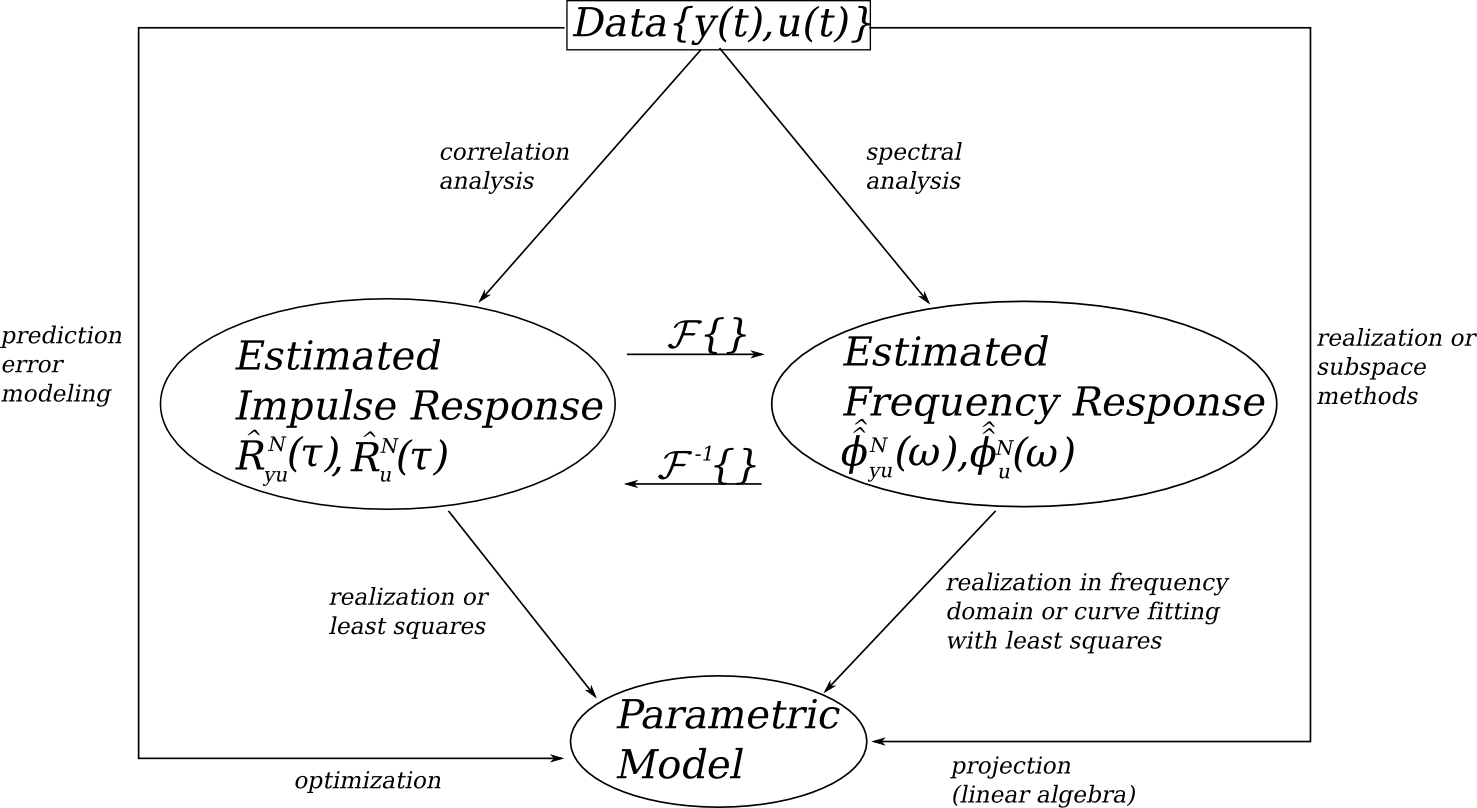
\includegraphics[width=1\textwidth]{images/07overview}
  \caption{Overview of parameter estimation.}
  \label{fig:07overview}
\end{figure}

Spectral analysis consists of
\begin{align*}
&\phiyuhat = \mathcal{F}\{\ryuhat\} = \frac{1}{N}Y_N(\w)U_N^*(\w) \\
&\lim_{N\to\infty}E\{\phiyuhat\} = \Phi_{yu}(\w) \text{ provided } \sum_{t=0}^\infty \tau|R_{yu}(\tau)| < \infty \\
&\lim_{N\to\infty}E\{[\phiyuhat - \Phi_{yu}(\w)]^2\} = \Phi_{yu}^2(\w)
\end{align*}
Additional averaging is needed to bring the variance to zero when using $\phiyuhat$. The new estimate with averaging included is
$$\phiyuhh = \frac{\int_{\xi=-\pi}^\pi \phiyuhat w(\w-\xi)d\xi}{\int_{\xi=-\pi}^\pi w(\xi)d\xi}$$
This is called the spectral estimate or spectral analysis.

How is all of this used? Starting with the system $y(t)=G_0(q)u(t)+v(t)$, with $v(t)=H_0(q)e(t)$ and $\{e(t)\}$ is white noise. This gives
\begin{align*}
\Phi_{yu}(\w) &= G_0(e^{j\w})\Phi_u(\w) + \Phi_{vu}(\w) \\
&= G_0(e^{j\w})\Phi_u(\w) \text{ if } u\perp v \\
\Rightarrow G_0(e^{j\w}) &= \frac{\Phi_{yu}(\w)}{\Phi_u(\w)} = \Phi_{yu}(\w)\Phi_u^{-1}(\w)
\end{align*}
The next step is to get a crude estimate of the transfer function using
$$\hat{G}(e^{j\w}) = \frac{\phiyuhat}{\phiuhat} = \frac{Y_N(\w)U_N^*(\w)}{U_N(\w)U_N^*(\w)} = \frac{Y_N(\w)}{U_N(\w)}$$
This is just dividing the transfer function of the output by the transfer function of the input. It is referred to as the empirical transfer function estimate (ETFE). Note that the means $\to 0$ but $\sigma>0$. The fact that the variance does not go to zero makes this a poor estimate. We can see this from the properties of $\phiyuhat$ and $\phiuhat$.
\begin{align*}
E\{\hat{G}(e^{j\w})\} &= G_0(e^{j\w}) \\
\text{var}\{\hat{G}(e^{j\w})\} &\nrightarrow 0 \text{ as } N\to\infty
\end{align*}
Also, remember Theorem 2.1 of Ljung.
\begin{align*}
y(t) &= G_0(q)u(t) + v(t) \\
Y_N(\w) &= G_0(e^{j\w})U_N(\w) + V_N(\w) + R_N(\w) \\
R_N(\w) &< 2\cdot \frac{1}{\sqrt{N}}\cdot C_w\cdot C_G \\
\frac{Y_N(\w)}{U_N(\w)} &= \hat{G}_0(e^{j\w}) = G_0(e^{j\w}) + \frac{V_N(\w)}{U_N(\w)} + \frac{R_N(\w)}{U_N(\w)}
\end{align*}
In the last equation there are separate terms for the variance due to noise and to end and beginning effects of the estimator.

It is possible to create an estimator that is better than the previous crude estimate by taking advantage of the spectral estimate.
\begin{align*}
\hat{\hat{G}}^N(e^{j\w}) &= \frac{\phiyuhh}{\phiuhh} = \frac{\int\hat{\Phi}_{yu}^N(\xi)w(\w-\xi)d\xi}{\int \hat{\Phi}_u^N(\xi)w(\w-\xi)d\xi} \\
E\{\ghh\} &= G(e^{j\w}) \\
\text{var}\{\hat{\hat{G}}(e^{j\w})\} &= 0 \text{ as } N\to\infty
\end{align*}
\textsc{Important:} Do some averaging by using this estimate based on the better spectral estimate. Include averaging on $\phiyuhat$, $\phiuhat$ to ensure a consistent estimate of $G_0(e^{j\w})$, the frequency response of the system. And note that this is \textit{not} a parametric model. That comes later.

\subsection{Averaging vs. Bias}
There will always be a trade-off between the amount of averaging done to reduce the variance and bias. See Figure \ref{fig:07msd} to see an example of a mass-spring-damper system and its frequency repsonse to a pulse input, $F(t)$. Note that the transfer function estimate is based on
$$\hat{\hat{G}}(e^{j\w}) = \frac{\int\hat{\Phi}_{Fx}^N(\xi)w(\w-\xi)d\xi}{\int \hat{\Phi}_F^N(\xi)w(\w-\xi)d\xi}$$
Here, $w(\xi)$ is a window or a weighting function. It will decrease the variance but it will also smooth out any real spikes in the frequency response. The smoothing feature leads to bias in the estimate. It is possible to use a window that is a function of frequency to reduce the bias but the trade-off will still exist. An example of the results that can be expected when using a very wide window is shown in Figure \ref{fig:07tradeoff}.

\begin{figure}[ht!]
  \centering
  \subfloat[Free-body diagram of mass spring damper system.]{
    \label{fig:07fbd}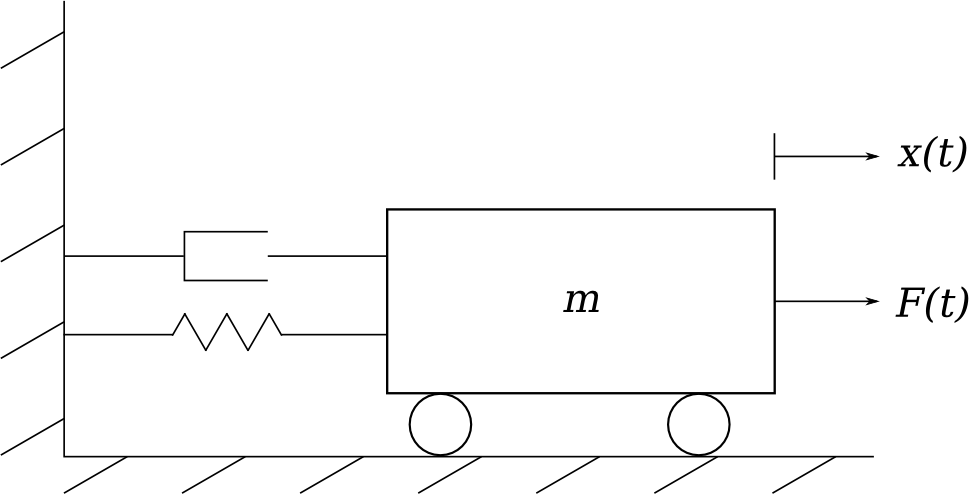
\includegraphics[width=0.4\textwidth]{images/07fbd}
  } \hfill
  \subfloat[Frequency response with variance.]{
    \label{fig:07freqResp}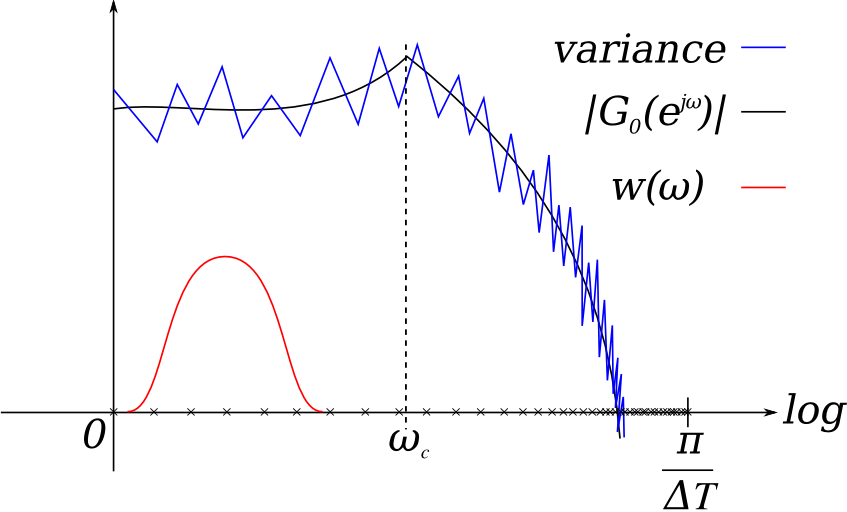
\includegraphics[width=0.4\textwidth]{images/07freqResp}
  } \hfill
  \caption{Frequency response of a mass spring damper system.}
  \label{fig:07msd}
\end{figure}

\begin{figure}[ht!]
  \centering
  \subfloat[Large variance, small bias.]{
    \label{fig:07largeSigma}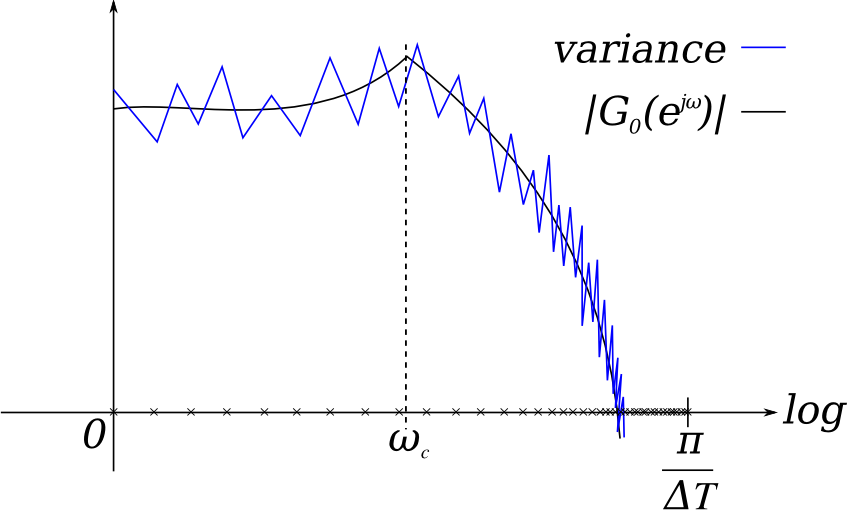
\includegraphics[width=0.4\textwidth]{images/07largeSigma}
  } \hfill
  \subfloat[Small variance, large bias.]{
    \label{fig:07smallSigma}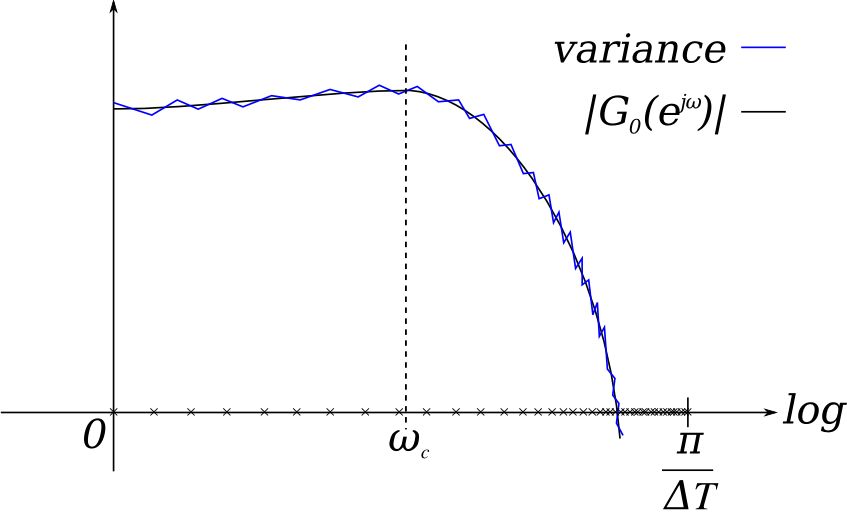
\includegraphics[width=0.4\textwidth]{images/07smallSigma}
  } \hfill
  \caption{Trade-off between variance and bias when averaging the spectrum.}
  \label{fig:07tradeoff}
\end{figure}

\subsection{Estimating Effects of Noise}
This corresponds to Chapter 6 in Ljung. Now that we have a method to get a nice estimate of the transfer function of the system, $G_0(q)$, we want to estimate a transfer function for the noise entering the system, $H_0(q)$. The transfer function of the noise shapes the spectrum of the noise signal. We are still using $v(t) = H_0(q)e(t)$, where $\{e(t)\}$ is white noise with unit variance. We know that
$$\Phi_v(\w) = |H_0(e^{j\w})|^2$$
How do we find the estimate $\hat{\Phi}_v(\w)$? One way would be to measure the output of the system with no inputs, or $\{u(t)\}=0 \Rightarrow y(t) = v(t) \Rightarrow \Phi_y(\w) = \Phi_v(\w)$. If $\{u(t)\}=0$ is not feasible then
\begin{align*}
\Phi_y(\w) &= |G_0(e^{j\w})|^2\Phi_u(\w) + \Phi_v(\w) \\
\Phi_v(\w) &= \Phi_y(\w) - |G_0(e^{j\w})|^2\Phi_u(\w) \\
&= \Phi_y(\w) - \frac{|\Phi_{yu}(\w)|^2}{\Phi_u(\w)}
\end{align*}
Now, suppose the estimate of the spectrum is
\begin{align*}
\hat{\hat{\Phi}}_v^N(\w) = \phiyhh - \frac{|\phiyuhh|^2}{\phiuhh} \Rightarrow \hat{\hat{\Phi}}_v(\w)\in\mathbb{R} = |H_0(e^{j\w})|^2
\end{align*}
Note that $\phiyhh\in\mathbb{R} = \mathcal{F}\{R_u(\tau)\}$ is real because $R_u(\tau)$ is symmetric and the Fourier transform of a symmetric signal is real. The same goes for $\phiuhh$. However, $\phiyuhh\in\mathbb{C}$ in general, but we are taking the square of that signal so it becomes real-valued as well. Using this result we can come up with a method for computing $H_0(e^{j\w})$, the frequency response of the transfer function of the noise entering the system, even when inputs are applied.

We start with
\begin{align*}
v(t) &= H_0(q)e(t) = \sum_{k=0}^\infty h_kq^{-k}e(t) \\
R_v(\tau) &= \sum_{k=0}^\infty h_kh_{k-\tau}
\end{align*}
From here we would like to get the impulse response coefficients, but this shows we can only get the product $h_kh_{k-\tau}$. This will only give us the frequency response squared. If we assume that $H_0(q)$ and $H_0^{-1}(q)$ are both stable and bounded then we can use spectral factorization to factor the product into two stable systems.

\begin{example}
Figure \ref{fig:07spectrum} shows an example of the spectrum of the noise signal. Then we have that
$$\Phi_v(\w) = |H_0(e^{j\w})|^2$$
Figure \ref{fig:07magphase}\subref{fig:07mag} shows the magnitude of the square root of the spectrum and Figure \ref{fig:07magphase}\subref{fig:07phase} shows the phase for the stable and unstable versions of the signal. This means that using $\sqrt{\Phi_v(\w)}$ lets the engineer choose a phase that yields a unique filter, $H_0(e^{j\w})$.
$\lozenge$
\end{example}

\begin{figure}[ht!]
  \centering
  \includegraphics[width=.5\textwidth]{images/07spectrum}
  \caption{Spectrum of the noise, $v(t)$.}
  \label{fig:07spectrum}
\end{figure}

\begin{figure}[ht!]
  \centering
  \subfloat[Magnitude of the spectrum.]{
    \label{fig:07mag}\includegraphics[width=0.4\textwidth]{images/07mag}
  } \hfill
  \subfloat[Phase of the spectrum.]{
    \label{fig:07phase}\includegraphics[width=0.4\textwidth]{images/07phase}
  } \hfill
  \caption{Magnitude and phase of the spectrum.}
  \label{fig:07magphase}
\end{figure}

\section{Linear Regression and Least Squares Method}
This corresponds to Chapter 7.3 of Ljung.

\subsection{Linear Regression Model}
When looking at discrete-time systems we can represent them as linear regression models (see \S\ref{sec:linearregression} for more details). The linear regression model looks like
$$y(t) = \varphi^T(t)\theta = \theta\varphi^T(t)$$
where
\begin{align*}
\phi^T(t) &= \left[\begin{array}{c c c c c c c c}
u(k) & u(k-1) & \cdots & u(k-n) & -y(k-1) & -y(k-2) & \cdots & -y(k-n) \end{array}\right] \\
\theta &= \left[\begin{array}{c c c c c c c c}
b_0 & b_1 & \cdots & b_n & a_1 & a_2 & \cdots & a_n \end{array}\right]^T
\end{align*}
This representation can easily be extended to non-linear systems even though it will still be linear in its parameter $\theta$.

The system is given by
$$\mathcal{S}: y(t) = \varphi^T(t)\theta_0$$
where $\theta_0$ is the ''real`` parameter. The model is
$$\mathcal{M}: y(t) = \varphi^T(t)\theta + e(t,\theta)$$
where $\theta$ is not necessarily $\theta_0$ but $\varphi(t)$ is the same between the system and the model. Notice that the model has an additional error term for when $\theta\neq\theta_0$. Note that $\varphi(t)$ is the set of all past inputs and outputs and $\theta$ contains the unknown parameters.

\subsection{Least Squares}
The objective of least squares is to find an estimate of the parameters such that
$$\hat{\theta} = \min_\theta\vectornorm{e(t,\theta)}_2^2 = \min_\theta e(t,\theta)e^T(t,\theta)$$
There are two ways to find a solution for the minimum: quadratic programming with equality constraints and minimizing a quadratic function that is linear in $\theta$. They both have unique minimums that can be explicityly computed. One method is to take the derivative and set it to zero and then solve. Another method is to use projection.

If we are given data $y(t),u(t),t=1,2,\ldots,N$, then we get
\begin{align*}
e(t,\theta) &= y(t) - \varphi^T(t)\theta \\
e(1,\theta) &= y(1) - \varphi^T(1)\theta \\
e(2,\theta) &= y(2) - \varphi^T(2)\theta \\
e(3,\theta) &= y(3) - \varphi^T(3)\theta \\
&\vdots
\end{align*}
Writing this out in matrix form gives
$$\underbrace{\mathbf{e}_N}_{N\times 1} = \underbrace{\mathbf{\Phi}}_{N\times p}\underbrace{\theta}_{p\times 1} - \underbrace{\mathbf{y}}_{N\times 1}$$
This leads to an estimation of the parameters as
$$\hat{\theta} = \min_\theta ||e(t,\theta)||_2^2 = \min_\theta \mathbf{e}_N^T\mathbf{e}_N$$

A geometric interpretation of this can be seen in Figure \ref{fig:07ls}. What we are attempting to do is project $\mathbf{e}$ orthogonally onto the parameter plane to get $\hat{\mathbf{y}}$. This leads to
\begin{align*}
\frac{1}{N}\vp^T(\mathbf{e} &= \mathbf{\vp}\mathbf{\theta} - \mathbf{y}) \\
\Rightarrow \frac{1}{N}\vp^Te &= \frac{1}{N}\vp^T\vp\theta - \frac{1}{N}\vp^Ty = 0 \\
\Rightarrow \hat{\theta}_{LS} &= \left(\frac{1}{N}\vp^T\vp\right)^{-1}\frac{1}{N}\vp^Ty
\end{align*}

\begin{figure}[ht!]
  \centering
  \includegraphics[width=.4\textwidth]{images/07ls}
  \caption{Least squares projection.}
  \label{fig:07ls}
\end{figure}

It is very interesting, and useful, to note that the term $\frac{1}{N}\varphi^Ty$ is the same as the cross-covariance function of the system and the term $\frac{1}{N}\varphi^T\varphi$ is the same as the auto-covariance function of the system.

%%%%%%%%%%%%%%%%%%%%%%%%%%%%%%%%%%%%%%%%%%%%%%%%%%%%%%%%%%%%%